  \documentclass[a4]{beamer}
\usepackage{amssymb}
\usepackage{graphicx}
\usepackage{subfigure}
\usepackage{newlfont}
\usepackage{amsmath,amsthm,amsfonts}
%\usepackage{beamerthemesplit}
\usepackage{pgf,pgfarrows,pgfnodes,pgfautomata,pgfheaps,pgfshade}
\usepackage{mathptmx} % Font Family
\usepackage{helvet} % Font Family
\usepackage{color}
\mode<presentation> {
\usetheme{Frankfurt} % was Frankfurt
\useinnertheme{rounded}
\useoutertheme{infolines}
\usefonttheme{serif}
%\usecolortheme{wolverine}
% \usecolortheme{rose}
\usefonttheme{structurebold}
}
\setbeamercovered{dynamic}
\title[MathsCast]{MathsCast Presentations \\ {\normalsize MA4413 Lecture 5B}}
\author[Kevin O'Brien]{Kevin O'Brien \\ {\scriptsize kevin.obrien@ul.ie}}
\date{Summer 2011}
\institute[Maths \& Stats]{Dept. of Mathematics \& Statistics, \\ University \textit{of} Limerick}
\renewcommand{\arraystretch}{1.5}
%------------------------------------------------------------------------%
\begin{document}
\begin{frame}
\titlepage
\end{frame}
%------------------------------------------%
\begin{frame}
\frametitle{Central Limit Theorem}
\begin{itemize}
\item The main aspect of the CLT that we shall consider is that many statistics (e.g sample mean and other related statistics, such as the sample variance) are normally distributed.
\item Consider the population, characterized by the histogram on the next slide.
\item While the population is not normally distributed, the population of sample statistic will be normally distributed.
\end{itemize}
\end{frame}
%------------------------------------------%
\begin{frame}
\frametitle{Central Limit Theorem}
\begin{figure}
  % Requires \usepackage{graphicx}
  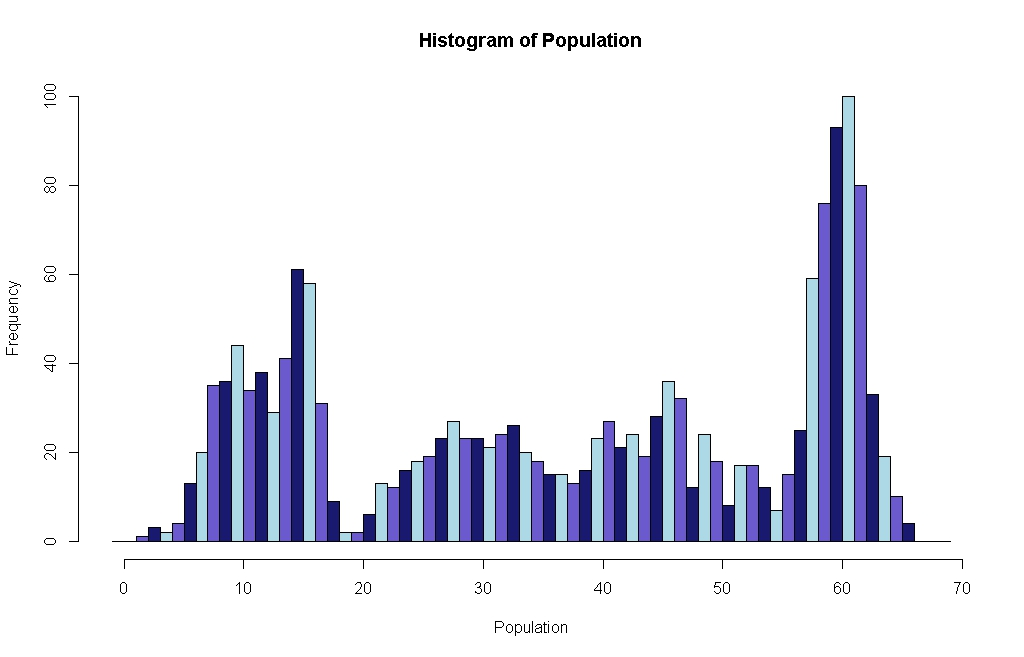
\includegraphics[scale=0.30]{images/6BPopHist}\\

\end{figure}

\end{frame}
%------------------------------------------%
\begin{frame}
\frametitle{Central Limit Theorem}
\begin{itemize}
\item Consider an experiment whereby a sample of 60 members of this population was taken, and the following sample statistics were computed
    \begin{itemize}
    \item Sample mean $\bar{X}$
    \item Sample variance $s^2$
    \item Sample median $\tilde{X}$
    \end{itemize}
\item This experiment was performed 100 times ( i.e. 100 independent samples were taken).
\item The sample statistics were collated by type and examined to determine normality.
\item A data set can be tested for normality using a very simple graphical procedure known as the `Normal Probability Plot', or Q-Q plot.
\item A data set can be assumed to be normally distributed if the points on the Q-Q plot follow the trendline.
\end{itemize}
\end{frame}
%------------------------------------------%
%------------------------------------------%
\begin{frame}
\frametitle{CLT: Sample Mean Q-Q plot}
\begin{figure}
  % Requires \usepackage{graphicx}
  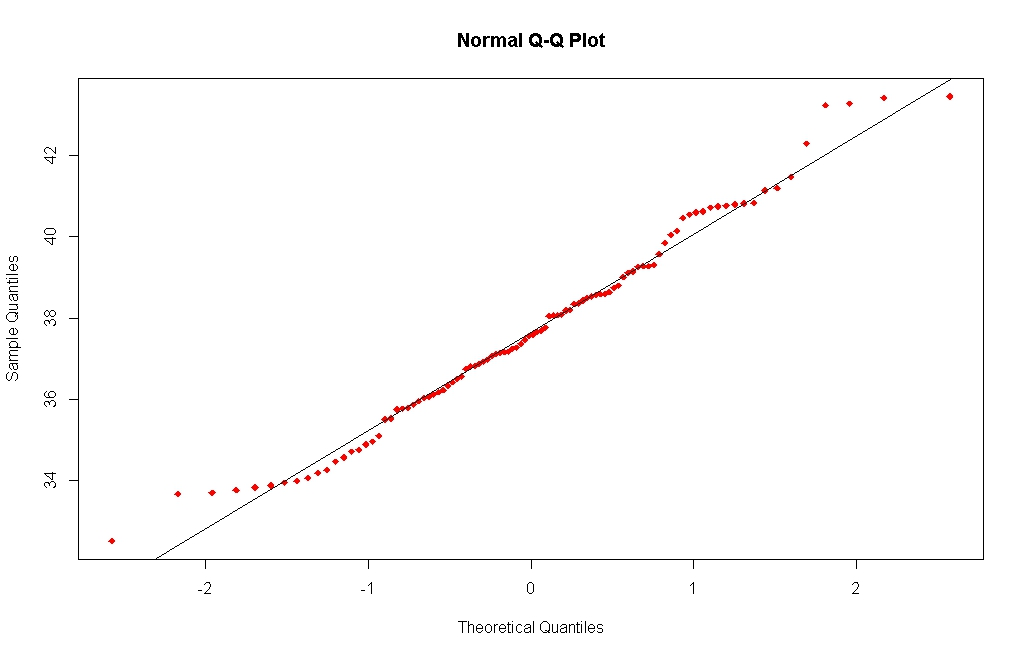
\includegraphics[scale=0.30]{images/6BmeanQQplot}\\

\end{figure}

\end{frame}
%------------------------------------------%
\begin{frame}
\frametitle{CLT: Sample Variance Q-Q plot}
\begin{figure}
  % Requires \usepackage{graphicx}
  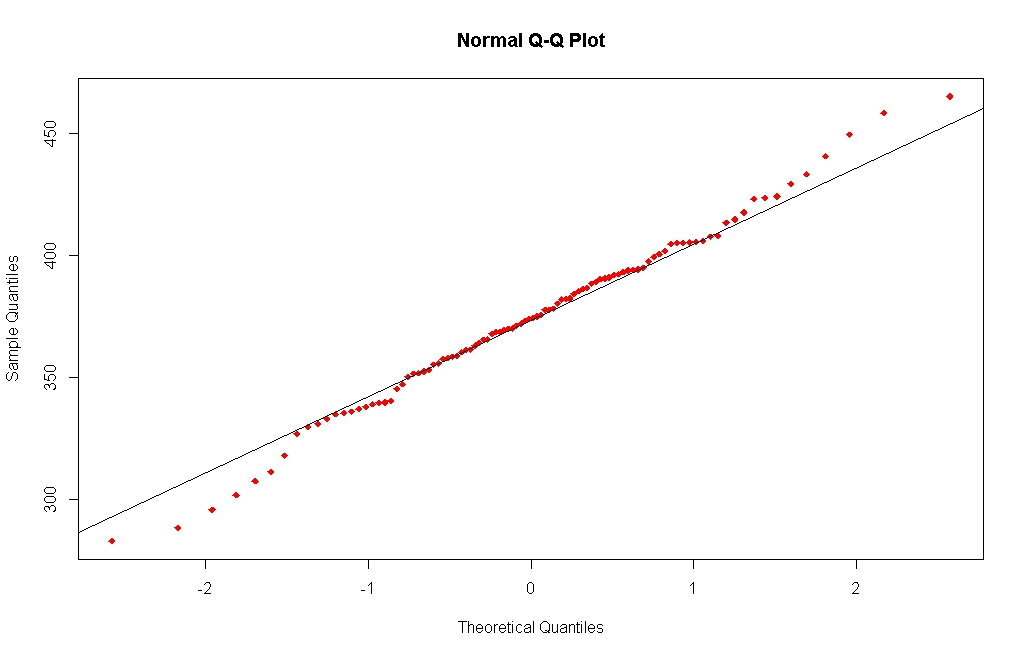
\includegraphics[scale=0.30]{images/6BvarQQplot}\\

\end{figure}

\end{frame}
%------------------------------------------%
\begin{frame}
\frametitle{CLT: Sample Median Q-Q plot}
\begin{figure}
  % Requires \usepackage{graphicx}
  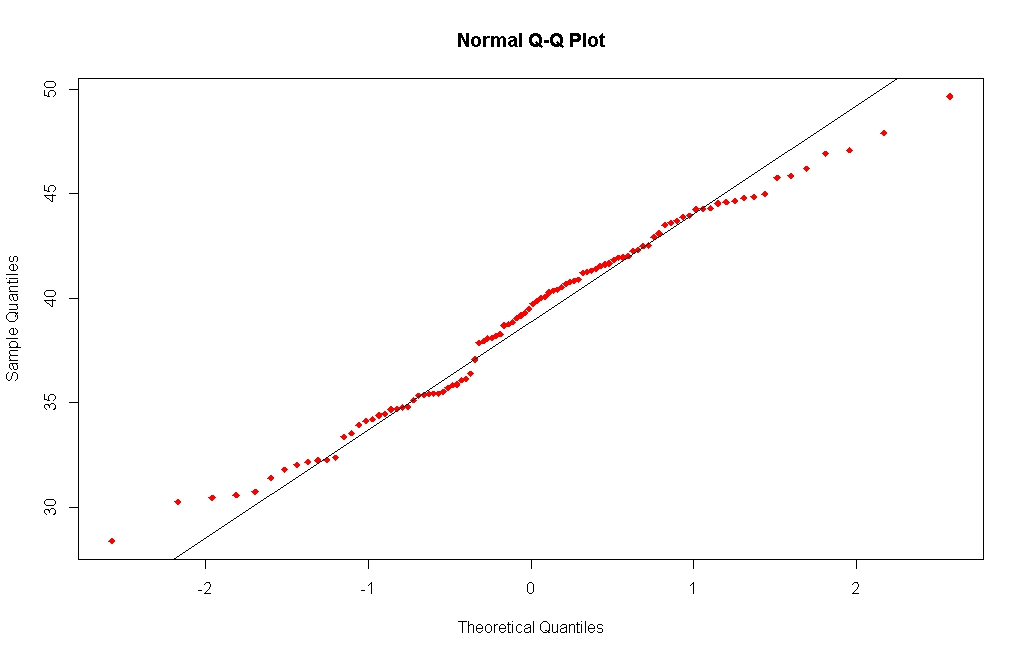
\includegraphics[scale=0.30]{images/6BmedianQQplot}\\

\end{figure}
\end{frame}
%------------------------------------------%
\begin{frame}
\frametitle{Central Limit Theorem: Sampling Distributions}
\begin{itemize}
\item In each of the three plots, the points follow the trend-line quite closely in each case.
\item As we can see, the population of these statistics are normally distributed.
\item We refer to these distributions as `Sampling Distributions'.
\item While the statistic that we will be dealing with in this module do have normal sampling distributions, it must be noted that many statistics have sampling distributions other than the normal distribution.
\end{itemize}
\end{frame}
%------------------------------------------%
\begin{frame}
\frametitle{Quantile Functions}
\begin{itemize} \item The Cumulative Distribution Function is used to identify the probability of a random variable being below a threshold value $k$.
\[P(X \leq k) \]

\item In short, we compute a probability values associated with a specified value.
\item (In \texttt{R}, this is carried out using the \texttt{p-} family of functions.)
\item With Quantile Functions, we are performing the opposite operation, i.e. for a specified probability, we determine the threshold value $k$.
\item For some value $p$, we computed $k$ such that
\[P(X \leq k) = p\]
\item (In \texttt{R}, this is performed using the \texttt{q-} family of functions.)
\end{itemize}

\end{frame}


%------------------------------------------%
\begin{frame}[fragile]
\frametitle{Quantile Functions}
\begin{itemize}
\item Recall that, from the Murdoch Barnes Tables, $P(Z \leq 1.96) = 0.975$ and $P(Z \leq 1.28) = 0.8997$
\end{itemize}
\begin{verbatim}
> qnorm(0.975)
[1] 1.959964
>
> qnorm(0.8997)
[1] 1.279844
\end{verbatim}
\end{frame}

\end{document}





Z = c(rnorm(300,10,3) , rnorm(150,15,1) , rnorm(100,24,3.5),rnorm(200,30,4) , rnorm(400,45,6),rnorm(500,60,2))
Population =Z
hist(Population, breaks = -1:69, col=c("midnightblue","lightblue","slateblue"))



Var.Sample = numeric()
Median.Sample = numeric()
Mean.Sample = numeric()

for( i in 1:100)
{
Sample = sample(Z,60)


Mean.Sample = c(Mean.Sample,mean(Sample))
Median.Sample = c(Median.Sample,median(Sample))
Var.Sample = c(Var.Sample,var(Sample))

}
qqnorm(Median.Sample, pch =18, col="red")
qqline(Median.Sample)
#
qqnorm(Mean.Sample, pch =18, col="red")
qqline(Mean.Sample)
#



qqnorm(Var.Sample, pch =18, col="red")
qqline(Var.Sample)

qqnorm(Median.Sample, pch =18, col="red")
qqline(Median.Sample)
